\documentclass[sigconf]{acmart} % , review

%% Import Packages
%\usepackage{times} % 会使得标题的字体改变
\usepackage{soul}
%\usepackage{url}
%\usepackage[utf8]{inputenc}
\usepackage{graphicx}
\usepackage{booktabs}
\usepackage{float}
\usepackage{overpic}
\usepackage{float}  %设置图片浮动位置的宏包
\usepackage{subfloat}
\usepackage{stfloats} % for pic
% \usepackage{subfigure}  %插入多图时用子图显示的宏包
\usepackage[skip=0.5\baselineskip]{caption}
\usepackage{bm}
\usepackage{amsmath}
%\usepackage{amsthm}
\usepackage{booktabs}
%\usepackage[switch]{lineno}
\usepackage{multirow}
\usepackage{multicol}
\usepackage{enumitem}
\usepackage{subcaption}
\usepackage{threeparttable}
\usepackage{xspace}
%\usepackage{amssymb}
\usepackage{color}
\usepackage[normalem]{ulem}
%\usepackage{algorithm}
%\usepackage{algorithmicx}
\usepackage{algorithmicx,algorithm}
\usepackage{algpseudocode}
\usepackage{algorithm,algpseudocode}
\usepackage{color, xspace}
\newcommand{\eg}[0]{\emph{e.g.,}\xspace}
\newcommand{\zxy}[1]{{\color{blue} [#1 – Xy]}}
\newcommand{\zc}[0]{{\color{blue} [cite]}\xspace}
\newcommand{\yc}[1]{{\color{purple}[yc: #1]}}
\newcommand{\xp}[1]{{\color{blue}[xp: #1]}}
\newcommand{\py}[1]{{\color{red}[py: #1]}}
\newcommand{\xdr}[1]{{\color{green}[xdr: #1]}}
\newcommand{\wl}[1]{{\color{orange}[wl: #1]}}
\newcommand{\edi}[1]{{\color{blue}{#1}}}
% for taxonomy figure drawing
\usepackage{color}
\usepackage{tikz}
\usepackage{xcolor}
\usepackage{xspace}
\usepackage{booktabs}
\usepackage{multirow}
\usepackage{makecell}
\usepackage[edges]{forest}

\AtBeginDocument{%
  \providecommand\BibTeX{{%
    \normalfont B\kern-0.5em{\scshape i\kern-0.25em b}\kern-0.8em\TeX}}}

\setcopyright{acmlicensed}
\copyrightyear{2023}
\acmYear{2023}
\acmDOI{XXXXXXX.XXXXXXX}

% \acmConference[KDD '25]{Proceedings of the 31th ACM SIGKDD Conference on Knowledge Discovery and Data Mining}{August 3--7, 2025}{Toronto, Canada}

% \acmISBN{978-1-4503-XXXX-X/18/06}

\begin{document}

\title{A Survey of Personalization: From RAG to Agent}
\author{Xiaopeng Li$^{1*}$, Pengyue Jia$^{1*}$, Derong Xu$^{1,3}$, Yi Wen$^1$, Yingyi Zhang$^{1,4}$, }
\author{Wenlin Zhang$^1$, Wanyu Wang$^1$, Yichao Wang$^{2}$, Xiangyang Li$^{2}$, Zhaocheng Du$^{2}$,}
\author{Yong Liu$^2$, Huifeng Guo$^2$, Ruiming Tang$^2$, Xiangyu Zhao$^1$}
\affiliation{
	\institution{$^1$City University of Hong Kong, $^2$Huawei Noah’s Ark Lab, \\ $^3$University of Science and Technology of China, $^4$Dalian University of Technology}
	\country{}
}
\email{{xiaopli2-c,jia.pengyue}@my.cityu.edu.hk, xianzhao@cityu.edu.hk}
\email{{wangyichao5, tangruiming}@huawei.com}
\thanks{* Equal contribution.}
% \email{xianzhao@cityu.edu.hk, {jt.g,yhwang25-c,xiaopli2-c,}@my.cityu.edu.hk}
% \email{liuqidong@stu.xjtu.edu.cn, {wangyichao5,chenbo116,huifeng.guo,tangruiming}@huawei.com}



\renewcommand{\shortauthors}{Xiaopeng Li and Pengyue Jia, et al.}

\begin{abstract}

Personalization has become an essential capability in modern AI systems, enabling customized interactions that align with individual user preferences, contexts, and goals. Recent research has increasingly concentrated on Retrieval-Augmented Generation (RAG) frameworks and their evolution into more advanced agent-based architectures within personalized settings to enhance user satisfaction. Building on this foundation, this survey systematically examines personalization across the three core stages of RAG: pre-retrieval, retrieval, and generation. Beyond RAG, we further extend its capabilities into the realm of Personalized LLM-based Agents, which enhance traditional RAG systems with agentic functionalities, including user understanding, personalized planning and execution, and dynamic generation. 
For both personalization in RAG and agent-based personalization, we provide formal definitions, conduct a comprehensive review of recent literature, and summarize key datasets and evaluation metrics. Additionally, we discuss fundamental challenges, limitations, and promising research directions in this evolving field. Relevant papers and resources are continuously updated at the Github Repo\footnote{\url{https://github.com/Applied-Machine-Learning-Lab/Awesome-Personalized-RAG-Agent}}.

\end{abstract}

% \begin{CCSXML}
% <ccs2012>
%    <concept>
%        <concept_id>10002951.10003317.10003338</concept_id>
%        <concept_desc>Information systems~Retrieval models and ranking</concept_desc>
%        <concept_significance>500</concept_significance>
%        </concept>
%    <concept>
%        <concept_id>10002951.10003227.10003351</concept_id>
%        <concept_desc>Information systems~Data mining</concept_desc>
%        <concept_significance>500</concept_significance>
%        </concept>
%  </ccs2012>
% \end{CCSXML}

% \ccsdesc[500]{Information systems~Retrieval models and ranking}
% \ccsdesc[500]{Information systems~Data mining}

\keywords{Large Language Model
(LLM), Retrieval-Augmented Generation (RAG), Agent, Personalization}
\vspace{-0.15in}

\settopmatter{printfolios=true}

\settopmatter{printacmref=false}
\renewcommand\footnotetextcopyrightpermission[1]{}

\maketitle

\section{Introduction}
Large Language Models (LLMs) have revolutionized AI-driven applications by enabling natural language understanding and generation at an unprecedented scale. However, these models often suffer from issues such as outdated responses and hallucinations, which severely hinder the accuracy of information generation. 
Retrieval-Augmented Generation (RAG) has emerged as a promising framework that integrates retrieved information from external corpora, such as external APIs~\cite{google,bing}, scientific repositories~\cite{arxiv,pubmed} or domain-specific databases~\cite{amazon_dataset, espn_dataset}, ensuring more knowledge-grounded and up-to-date outputs. 

Its versatility has led to significant applications across various domains, including question answering~\cite{siriwardhana2023improving}, enterprise search~\cite{bulfamante2023generative} and healthcare~\cite{wu2024medical}, etc. Among these applications, one particularly notable area is in agent workflows, where RAG enhances autonomous systems by providing context-aware, dynamically retrieved, and reliable knowledge. This is because each stage of the RAG process closely mirrors key aspects of an agent’s workflow, as shown in Figure~\ref{fig:structure}. For instance, the query rewriting phase in RAG, which involves semantic understanding and parsing, aligns with the semantic comprehension stage in agent workflows. Likewise, RAG’s retrieval phase, which focuses on extracting the most relevant documents, corresponds to the planning and execution phases of an agent, where decisions are made based on retrieved knowledge. Finally, the generation phase in RAG parallels an agent’s execution stage, where actions are performed based on the given task. This structural alignment suggests that the architecture of RAG is fundamentally converging with agent workflows, solidifying its position as a key facilitator of intelligent and autonomous systems.

Although the structural alignment between RAG and agent workflows highlights their deepening convergence, a critical next step in enhancing these intelligent systems lies in personalization. Personalization is a key driver toward achieving more adaptive and context-aware AI, which is fundamental for the progression toward Artificial General Intelligence (AGI). It plays an essential role in applications such as personalized reasoning~\cite{xu2021transformer, henze2004reasoning}, adaptive decision-making~\cite{lu2011budgeted}, user-specific content generation~\cite{xu2025personalized, shaker2010towards}, and interactive AI systems~\cite{ma2021one, qian2021learning}. However, existing research lacks a comprehensive comparative analysis of personalized RAG and agentic approaches. Current surveys primarily focus on general RAG methodologies~\cite{gao2023retrieval, fan2024survey} or agent-related literature~\cite{li2024personal, wang2024survey, zhang2024survey}, without systematically exploring their implications for personalization. While recent works such as~\cite{zhang2024personalization, liu2025survey} discuss personalization, they predominantly address personalized generation within LLMs or specific downstream tasks, overlooking how personalization can be effectively integrated into RAG and agent workflows.

Motivated by the above issues, this survey aims to provide a comprehensive review of the integration of personalization into RAG and agentic RAG frameworks to enhance user experiences and optimize satisfaction. The key contributions of this work can be summarized as follows:
\begin{itemize}[leftmargin=*] 
\item We provide an extensive exploration of the existing literature on how personalization is integrated into various stages of RAG (pre-retrieval, retrieval, and generation) and agentic RAG (understanding, planning, execution, and generation).
\item We summarize the key datasets, benchmarks, and evaluation metrics used in existing research for each subtask to facilitate future studies in the respective domains. 
\item We also highlight the limitations of current research and suggest future directions for personalized RAG, emphasizing potential advancements to address existing challenges.
\end{itemize}


The outline of this survey is as follows: we introduce what is personalization (Sec.~\ref{sec:what}) and explain how personalization is adopted into RAG pipeline (Sec.~\ref{sec:how}). Then, we present a literature review on where to integrate personalization within different stages of RAG and agentic RAG workflows~(Sec.~\ref{sec:where}) and discuss the key datasets and evaluation metrics used in existing research~(Sec.\ref{sec:evaluation&dataset}). Lastly, we present a discussion on the limitations of current research and future directions~(Sec.~\ref{sec:futuredirection}).

\begin{figure}[t]
    \centering
    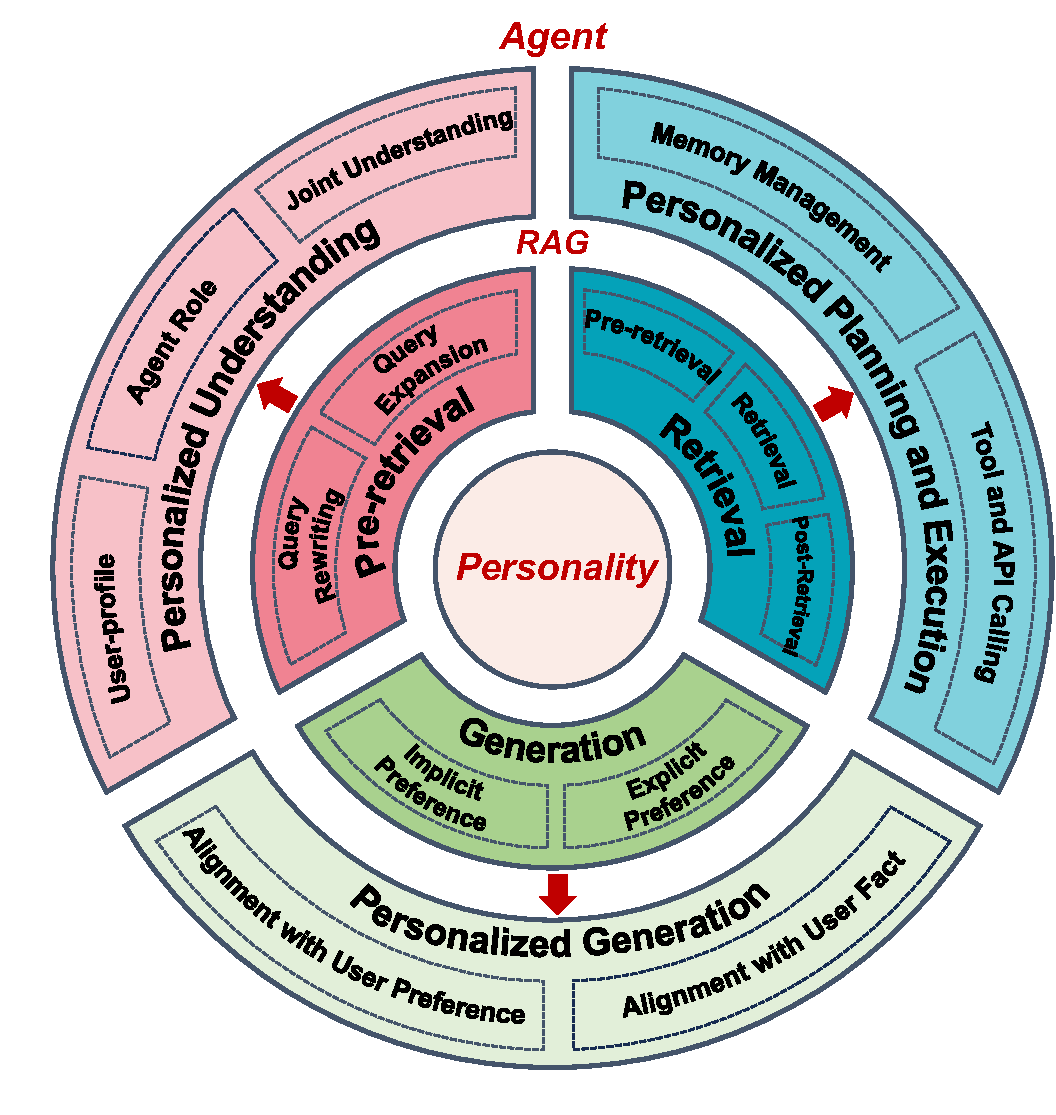
\includegraphics[width = 0.6\linewidth]{figures/structure.pdf}
    \caption{Correlation between personalization and RAG with agent flow.}
    \label{fig:structure}
\end{figure}

\begin{table*}[t]
% \setlength\tabcolsep{3pt}  %可以控制列间距
% \renewcommand{\arraystretch}{1} %可以控制行间距
\caption{Overview of Personalized RAG and Agent.}
\centering
\resizebox{\textwidth}{!}{
\begin{tabular}{c|c|c|c} 
\toprule
\textbf{Field}                              & \textbf{Sub-field}                                                                                       & \textbf{Subsub-field}                                                                          & \textbf{Papers}                                                                                                                                                                                                                                                                                                                                                                                                                                                                                                                                                                                                                                                                                                                                                                                                                                            \\ 
\midrule
\multirow{7}{*}{\textbf{Pre-retrieval}}     & \multirow{4}{*}{\begin{tabular}[c]{@{}c@{}}Query\\Rewriting\end{tabular}}                       & \begin{tabular}[c]{@{}c@{}}Learning to\\Personalized Query Rewrite\end{tabular}          & CLE-QR \cite{li2022query}, CGF \cite{hao2022cgf}, PEARL \cite{mysore2023pearl}                                                                                                                                                                                                                                                                                                                                                                                                                                                                                                                                                                                                                                                                                                                 \\ 
\cmidrule{3-4}
                                   &                                                                                                 & \begin{tabular}[c]{@{}c@{}}LLM to\\Personalized Query Rewrite\end{tabular} & Least-to-Most Prompting \cite{zhou2022least}, ERAGent \cite{shi2024eragent}, CoPS \cite{zhou2024cognitive}, Agent4Ranking \cite{li2023agent4ranking}, FIG \cite{chen2023graph}, BASES \cite{ren2024bases}                                                                                                                                                                                                                                                                                                                                                                                                                                                                                                                                  \\ 
\cmidrule{2-4}
                                   & \multirow{3}{*}{\begin{tabular}[c]{@{}c@{}}Query\\Expansion\end{tabular}}                       & \begin{tabular}[c]{@{}c@{}}Tagging-based query\\expansion\end{tabular}                & Gossple~\cite{bertier2009toward}, ~\citet{biancalana2009social}, SoQuES~\cite{bouadjenek2011personalized}, ~\citet{zhou2012improving}                                                                                                                                                                                                                                                                                                                                                                                                                                                                                                                                                                         \\ 
\cmidrule{3-4}
                                   &                                                                                                 & Else                                                                                  & ~\citet{lin2006personalized}, ~\citet{bender2008exploiting}, Axiomatic PQEC~\cite{mulhem2016axiomatic}, WE-LM~\cite{wu2017personalized}, PSQE~\cite{bouadjenek2019personalized}, PQEWC~\cite{bassani2023personalized}                                                                                                                                                                                                                                                                                                                                                                                                                       \\ 
\cmidrule{2-4}
                                   & \multicolumn{2}{c|}{Others}                                                                                                                                                             & Bobo~\cite{gao2010utilizing}, ~\citet{kannadasan2019personalized}, PSQE~\cite{baumann2024psqe}                                                                                                                                                                                                                                                                                                                                                                                                                                                                                                                                                                                                                                                 \\ 
\midrule
\multirow{9}{*}{\textbf{Retrieval}}         & \multicolumn{2}{c|}{Indexing}                                                                                                                                                           & PEARL~\cite{mysore2023pearl}, KG-Retriever~\cite{chen2024kg}, EMG-RAG~\cite{wang2024crafting}, PGraphRAG~\cite{au2025personalized}                                                                                                                                                                                                                                                                                                                                                                                                                                                                                                                                                                                                                                                                                                                                                                                                     \\ 
\cmidrule{2-4}
                                   & \multirow{7}{*}{Retrieval}                                                                       & \begin{tabular}[c]{@{}c@{}}Dense\\Retrieval\end{tabular}                               & \begin{tabular}[c]{@{}c@{}}MeMemo \cite{wang2024mememo}, RECAP \cite{liu2023recap}, LAPDOG \cite{huang2024learning}, \citet{gu2021partner}, PersonaLM \cite{mathur2023personalm}, UIA \cite{zeng2023personalized}, XPERT \cite{vemuri2023personalized}, DPSR \cite{zhang2020towards}, \\RTM \cite{bi2021learning}, Pearl \cite{mysore2023pearl}, MemPrompt \cite{madaan2022memory}, ERRA \cite{cheng2023explainable}, MALP \cite{zhang2023llm}, USER-LLM \cite{ning2024user}, PER-PCS \cite{tan2024personalized}\end{tabular}                                                      \\ 
\cmidrule{3-4}
                                   &                                                                                                 & \begin{tabular}[c]{@{}c@{}}Sparse\\Retrieval\end{tabular}                              & OPPU \cite{tan2024democratizing}, PAG \cite{richardson2023integrating}, \citet{au2025personalized}, UniMS-RAG \cite{wang2024unims}, \citet{deng2022toward},                                                                                                                                                                                                                                                                                                                                                                                                                                                                                                                                                                                                  \\ 
\cmidrule{3-4}
                                   &                                                                                                 & \begin{tabular}[c]{@{}c@{}}Prompt-based\\Retrieval\end{tabular}                        & LAPS \cite{joko2024doing}, UniMP \cite{wei2024towards}, \citet{shen2024heart}                                                                                                                                                                                                                                                                                                                                                                                                                                                                                                                                                                                                                                                                                                                  \\ 
\cmidrule{3-4}
                                   &                                                                                                 & Others                                                                                & \citet{salemi2024optimization}, PersonalTM \cite{lian2023personaltm}, \citet{zhang2024personalized}                                                                                                                                                                                                                                                                                                                                                                                                                                                                                                                                                                                                                                                                                            \\ 
\cmidrule{2-4}
                                   & \multicolumn{2}{c|}{Post-retrieval}                                                                                                                                                      & PersonaRAG~\cite{zerhoudi2024personarag}, \citet{pavliukevich2024improving}, UniMS-RAG~\cite{wang2024unims}, \citet{salemi2024learning}, \citet{zhang2025rehearse}, AutoCompressors~\cite{chevalier2023adapting}, FIT-RAG~\cite{mao2024fit}                                                                                                                                                                                                                                                                                                                                                                                                                                                                                                                                                                                                                                                                                                                                                                \\ 
\midrule
\multirow{11}{*}{\textbf{Generation}}        & \multirow{6}{*}{\begin{tabular}[c]{@{}c@{}}Generation from\\Explicit Preferences\end{tabular}}  & \begin{tabular}[c]{@{}c@{}}Direct\\Prompting\end{tabular}                             & P$^2$~\cite{jiang2023evaluating}, Character Profiling~\cite{yuan2024evaluating}  OpinionQA~\cite{santurkar2023whose}, ~\citet{kang2023llms}, ~\citet{liu2023chatgpt}, Cue-CoT~\cite{wang2023cue}, TICL~\cite{cho2025tuning}                                                                                                                                                                                                                                                                                                                                                                           \\ 
\cmidrule{3-4}
                                   &                                                                                                 & \begin{tabular}[c]{@{}c@{}}Profile-Augmented\\Prompting\end{tabular}                  & GPG~\cite{zhang2024guided}, ~\citet{richardson2023integrating}, ONCE~\cite{liu2024once}, LLMTreeRec~\cite{zhang2025llmtreerec}, KAR~\cite{xi2024towards}, Matryoshka~\cite{li2024matryoshka}                                                                                                                                                                                                                                                                                                                                                                                                                                                \\ 
\cmidrule{3-4}
                                   &                                                                                                 & \begin{tabular}[c]{@{}c@{}}Personalized-Prompt\\Prompting\end{tabular}                & \citet{li2024learning}, RecGPT~\cite{zhang2024recgpt}, PEPLER-D~\cite{li2023personalized}, GRAPA~\cite{qu2024graph}, SGPT~\cite{deng2024unlocking}, PFCL~\cite{yu2024personalized}                                                                                                                                                                                                                                                                                                                                                                                                                                                                          \\ 
\cmidrule{2-4}
                                   & \multirow{4}{*}{\begin{tabular}[c]{@{}c@{}}Generation from \\Implicit Preferences\end{tabular}} & \begin{tabular}[c]{@{}c@{}}Fine-tuning-Based\\Methods\end{tabular}                    & \begin{tabular}[c]{@{}c@{}}PLoRA~\cite{zhang2024personalized}, LM-P~\cite{wozniak2024personalized}, MiLP~\cite{zhang2024personalized}, OPPU~\cite{tan2025democratizing}, PER-PCS~\cite{tan2024personalized}, Review-LLM~\cite{peng2024reviewllm},\\UserIdentifier~\cite{mireshghallah2021useridentifier}, UserAdapter~\cite{zhong2021useradapter}, HYDRA~\cite{zhuang2406hydra}, PocketLLM~\cite{peng2024pocketllm}, CoGenesis~\cite{zhang2024cogenesis}\end{tabular}  \\ 
\cmidrule{3-4}
                                   &                                                                                                 & \begin{tabular}[c]{@{}c@{}}Reinforcement\\Learning-Based\\Methods\end{tabular}        & P-RLHF~\cite{li2024personalized}, P-SOUPS~\cite{jang2023personalized}, PAD~\cite{chen2024pad}, REST-PG~\cite{salemi2025reasoning}, \citet{salemi2024optimization}, RewriterSlRl~\cite{li2024learning},\citet{kulkarni2024reinforcement}                                                                                                                                                                                                                                                                                                                                                                                                    \\ 
\midrule
\multirow{13}{*}{\textbf{From RAG to Agent}} & \multirow{6}{*}{\begin{tabular}[c]{@{}c@{}}Personalized\\Understanding\end{tabular}}            & \begin{tabular}[c]{@{}c@{}}In user-profile\\understanding\end{tabular}                & \citet{xu2024penetrative}, \citet{abbasian2023conversational},                                                                                                                                                                                                                                                                                                                                                                                                                                                                                                                                                                                                                                                                                                                                                  \\ 
\cmidrule{3-4}
                                   &                                                                                                 & \begin{tabular}[c]{@{}c@{}}In agent’s role\\understanding\end{tabular}                & RoleLLM~\cite{wang2023rolellm}, Character-LLM~\cite{shao2023character}, \citet{wang2023incharacter},                                                                                                                                                                                                                                                                                                                                                                                                                                                                                                                                                                                                                                                           \\ 
\cmidrule{3-4}
                                   &                                                                                                 & \begin{tabular}[c]{@{}c@{}}In agent’s user-role\\joint understanding\end{tabular}     & SocialBench \cite{chen2024socialbench}, \citet{dai2024mmrole}, \citet{ran2024capturing}, \citet{wang2023enabling}, \citet{tu2024charactereval}, Neeko \cite{yu2024neeko}                                                                                                                                                                                                                                                                                                                                                                                                                                                                                                                                                                    \\ 
\cmidrule{2-4}
                                   & \multirow{2}{*}{\begin{tabular}[c]{@{}c@{}}Personalized Planning\\and Execution\end{tabular}}   & \begin{tabular}[c]{@{}c@{}}Memory\\Management\end{tabular}                            & EMG-RAG \cite{wang2024crafting}, \citet{park2023generative}, \citet{abbasian2023conversational}, RecAgent \cite{wang2023user}, TravelPlanner+ \cite{singh2024personal}, PersonalWAB \cite{cai2025large}, VOYAGER \cite{wangvoyager}, MemoeryLLM \cite{wangmemoryllm}                                                                                                                                                                                                                                                                                                                                                                                                                                                                                                                                                                                      \\ 
\cmidrule{3-4}
                                   &                                                                                                 & Tool and API Calling                                                                  & VOYAGER \cite{wangvoyager}, \citet{zhangbootstrap}, PUMA \cite{cai2025large}, \citet{wang2023enabling}, PenetrativeAI \cite{xu2024penetrative}, \citet{huang2022language}, \cite{park2023generative}, MetaGPT \cite{hong2023metagpt}, OKR-Agent \cite{zheng2023agents}                                                                                                                                                                                                                                                                                                                                                                                                                                                                                                                                                                                                                                                                        \\ 
\cmidrule{2-4}
                                   & \multirow{4}{*}{\begin{tabular}[c]{@{}c@{}}Personalized\\Generation\end{tabular}}               & \begin{tabular}[c]{@{}c@{}}Alignment with \\User Fact\end{tabular}                   & Character-LLM \cite{shao2023character}, \citet{wang2024investigating}, \citet{dai2024mmrole}                                                                                                                                                                                                                                                                                                                                                                                                                                                                                                                                                                                                                                                                                                   \\ 
\cmidrule{3-4}
                                   &                                                                                                 & \begin{tabular}[c]{@{}c@{}}Alignment with User\\Preferences\end{tabular}              & \citet{wang2023rolellm}, \citet{ran2024capturing}, \citet{wang2023incharacter}, \citet{chen2024socialbench}                                                                                                                                                                                                                                                                                                                                                                                                                                                                                                                                                                                                                                                                   \\
\bottomrule
\end{tabular}}
\end{table*}

\section{What is Personalization} \label{sec:what}
Personalization in current research refers to the tailoring of model predictions or generated content to align with an individual's preferences. In the context of RAG and agents, personalization involves incorporating user-specific information at various stages of the RAG pipeline or within agents. User personalization can be categorized into the following types:

\begin{itemize}[leftmargin=*] 
\item Explicit User Profile: Explicitly presented user information, including biographical details, attributes (\eg age, location, gender, education), and social connections (\eg social networks).
\item User Historical Interactions: Behavioral data, including browsing history, clicks, and purchases, which help infer user interests and preferences to improve personalization. 
\item User Historical Content: Implicit personalization derived from user-generated content, such as chat history, emails, reviews, and social media interactions. 
\item Persona-Based User Simulation: The use of LLM-based agents to simulate and generate personalized interactions.
\end{itemize}

Integrating this personalized information at various stages of the RAG and agent workflows enables dynamic alignment with human preferences, thereby making responses more user-centric and adaptive.
\section{How to Adopt Personalization} \label{sec:how}
We define the process of introducing personalization within the RAG pipeline as follows:
% \vspace{-1mm}
\begin{equation}\label{equ:definition}
g = \mathcal{G} \left( \mathcal{R}\left(\mathcal{Q}\left(q,p\right),\mathcal{C},p\right),\text{prompt},p,\theta \right)
\end{equation}
% \vspace{-1mm}
where $p$ denotes personalized information, and the process unfolds in three steps. In the \textbf{pre-retrieval phase}, query processing ($\mathcal{Q}$) refines the query $q$ using personalized information, such as through query rewriting or expansion. During the \textbf{retrieval phase}, the retriever ($\mathcal{R}$) leverages $p$ to fetch relevant documents from the corpus ($\mathcal{C}$). Finally, in the \textbf{generation phase}, the retrieved information, combined with $p$ and structured using the given prompt, id fed into the generator ($\mathcal{G}$) with parameter $\theta$ to produce the final response $g$. It is evident that personalized information directly influences multiple stages of the RAG pipeline. In this survey, we consider the agent system as a specialized application of the RAG framework, where personalization is incorporated in a manner similar to the RAG framework.
\input{4.1Where pre-retrieval}
\input{4.2Where retrieval}
\input{4.3Where generation}
\input{4.4Where agent}
\input{5Evaluation and Dataset}
\input{6Future Direction}
\section{Conclusion}
In this paper, we explore the landscape of personalization from Retrieval-Augmented Generation (RAG) to advanced LLM-based Agents, detailing adaptations across pre-retrieval, retrieval, and generation stages while extending into agentic capabilities. By reviewing recent literature, datasets, and metrics, we highlight the progress and diversity in enhancing user satisfaction through tailored AI systems. 
However, challenges such as scalability, effective evaluation, and ethical concerns underscore the need for innovative solutions. Future research should focus on lightweight frameworks, specialized benchmarks, and privacy-preserving techniques to advance personalized AI. 
Relevant papers and resources are also compiled online for ease of future research.


\bibliographystyle{ACM-Reference-Format}
\bibliography{newbibfile}


\end{document}
